\chapter{Wiring e o AVR}

\section{Atmel AVR}

O AVR é um microcontrolador RISC desenvolvido pela Atmel e posteriormente comprado pela Microchip Tecnology. Possui uma pequena memória flash para armazenamento do programas e 32 registradores internos. Este tipo de chip é muito utilizado em hardwares de prototipagem, como o Arduíno.

Conforme \citeonline{borges2006desenvolvimento} "Com o objetivo de maximizar o desempenho e o paralelismo, o AVR segue arquitetura Harvard, em que os barramentos associados às memórias de dados e do programa são distintos. Além disso, utiliza-se a técnica do \emph{pipeline}, em que, enquanto uma instrução começa a ser executada, uma outra já é buscada na memória de programa para que a mesma possa ser executada no próximo ciclo de relógio"

Um microcontrolador possui internamente todas as características de um computador possuindo processador, memória e periféricos de entrada e saída. Este tipo de circuito é conhecido como \emph{System-on-chip}\footnote{\url{https://pt.wikipedia.org/wiki/System-on-a-chip}}. Esta característica o faz ser amplamente utilizado em hardwares de prototipagem pois possui características suficientes para a execução de programas e acionamento de pinos, por exemplo.

A versão mais popular do Arduíno, o Arduíno Uno, possui um microcontrolador ATmega328 (\autoref{atmega})

\begin{figure}[htb]
	\begin{center}
	    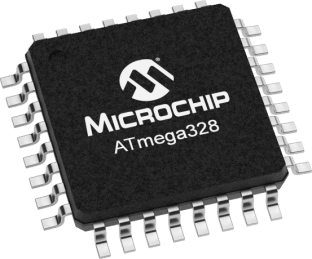
\includegraphics[scale=0.5]{artigo/refs/medium-ATmega328-TQFP-32.png}
	\end{center}
	\caption{\label{atmega}chip ATmega328}
	%\legend{Fonte: Site da 3GPP}
\end{figure}

Algumas das características do ATmega328 são listadas na tabela abaixo

\section{Programando para AVR}

No diretório de instalação do Arduíno há uma biblioteca denominada avr/io.h, esta biblioteca possui todas as diretivas para outras bibliotecas com base no microcontrolador utilizado. Nestas bibliotecas há definições de registradores de entrada e saída, pinos, constantes e diversos outros componentes, conforme trecho abaixo.

\subsection{Bibliotecas AVR}

Aqui um pequeno trecho da biblioteca io.h em que, de acordo com o chip AVR utilizado, uma nova biblioteca é incluída.

\begin{lstlisting}
//biblioteca io.h
//(...)
#ifndef _AVR_IO_H_
#define _AVR_IO_H_

#include <avr/sfr_defs.h>

#if defined (__AVR_AT94K__)
#  include <avr/ioat94k.h>
//(...)
#elif defined (__AVR_ATmega328P__)
#  include <avr/iom328p.h>
#elif (defined __AVR_ATmega328__)
#include <avr/iom328.h>
//(...)

\end{lstlisting}
%INSERIR IMAGEM DO ATMEGA328, INSERIR TAMBÉM UM TRECHO OU OUTRO E FINALIZAR

Aqui um pequno trecho da biblioteca io.h em que, de acordo com o chip AVR utilizado, uma nova biblioteca é incluída.

\begin{lstlisting}
//biblioteca iom328p.h
//(...)
#ifndef _AVR_IOM328P_H_
#define _AVR_IOM328P_H_ 1

/* Registers and associated bit numbers */

#define PINB _SFR_IO8(0x03)
#define PINB0 0
//(...)
#define DDRB _SFR_IO8(0x04)
#define DDB0 0
#define DDB1 1
//(...)
#define PORTB _SFR_IO8(0x05)
#define PORTB0 0
#define PORTB1 1
//(...)
\end{lstlisting}
